\documentclass{beamer}
\usepackage{polski}
\usepackage[polish]{babel}
\usepackage[utf8]{inputenc}
\usepackage{default}

\usepackage[style=authortitle,backend=biber]{biblatex}
\addbibresource{bibliografia.bib}

\title{Git}
\author{Marta Sawko}
\usetheme{Singapore}
\usecolortheme{dove}

\usepackage{xcolor}
\usepackage{listings}
\usepackage{caption}
\DeclareCaptionFont{white}{\color{white}}
\DeclareCaptionFormat{listing}{%
  \parbox{\textwidth}{\colorbox{gray}{\parbox{\textwidth}{#1#2#3}}\vskip-4pt}}
\captionsetup[lstlisting]{format=listing,labelfont=white,textfont=white}
\lstset{frame=lrb,xleftmargin=\fboxsep,xrightmargin=-\fboxsep}

\begin{document}

\frame{\titlepage}
\begin{frame}{Plan seminarium}
  \tableofcontents
\end{frame}

\begin{frame}
 \frametitle{System kontroli wersji}
 \framesubtitle{\textbf{V}ersion \textbf{C}ontrol \textbf{S}ystem}
 Jest to oprogramowanie, pozwalające na szeroko rozumiane nadzorowanie zmian w plikach w czasie, np.:
 \begin{itemize}
  \item badania zmian w obrębie konkretnych fragmentów tekstu, jak linijki
  \item powrotu do wcześniejszych wersji 
  \item w pracy grupowej - znajdowanie winnego powstałych zmian
 \end{itemize} 
 Pierwszy pomysł na rozwiązanie - Local Control Version System.
\end{frame}

\section{Centalizacja a rozproszenie}
\subsection{Centralizacja}
\begin{frame}{\textbf{C}entral \textbf{V}ersion Control \textbf{S}ystems}
  Zlokalizowane w jednym miejscu. (tzn gdzie, serwer?) \\
  Posiadając pewne uprawnienia można wiedzieć dokładnie co kto robi.\\
  \begin{center}
   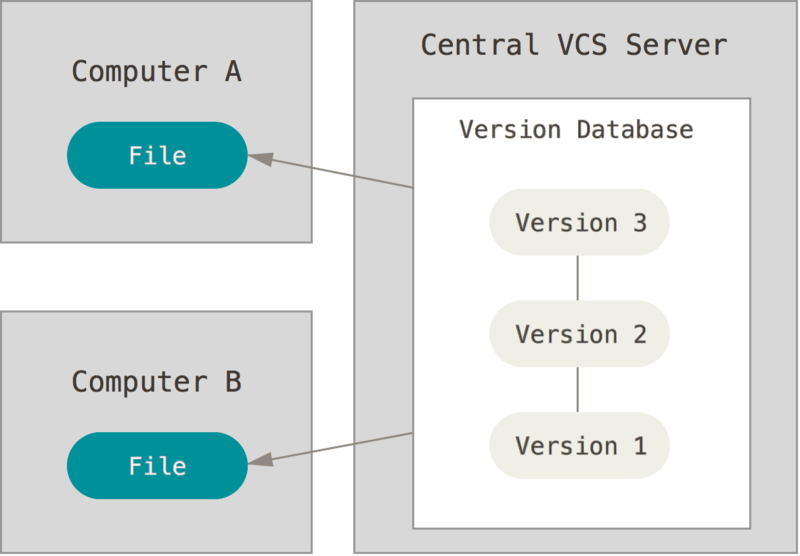
\includegraphics[height=0.4\textwidth]{./obrazki/fig-1_2.png}
   \footfullcite{pro_git}
 \end{center}
  Przykładowe CVS\@: \textit{Subversion}, \textit{Perforce}
\end{frame}

\begin{frame}
  Potencjalne wady CVS:\@
  \begin{itemize}
  \item kiedy pada centralny serwer, zaniechana jest praca nad projektem
  \item kiedy padnie sieć współpracownika, zaniechana jest jego praca nad projektem
  \item kiedy pada centralny dysk, na którym wszyscy pracują, to tracimy wszystkie dane 
 \end{itemize}
\end{frame}

\subsection{Dystrybucja}
\begin{frame}
 \frametitle{\textbf{D}istributed \textbf{V}ersion \textbf{C}ontrol \textbf{S}ystems}
  Każdy klon jest pełną kopią danych i stanowi oddzielne kompletne repozytorium.\\
  Czynności takie jak przeglądanie historii, \textit{commit} są szybkie, bo nie wymagają połączenia z serwerem.
\\
 Przykłady DVCs: \textit{Git, Mercurial}
\end{frame}

\begin{frame}
  \begin{center}
   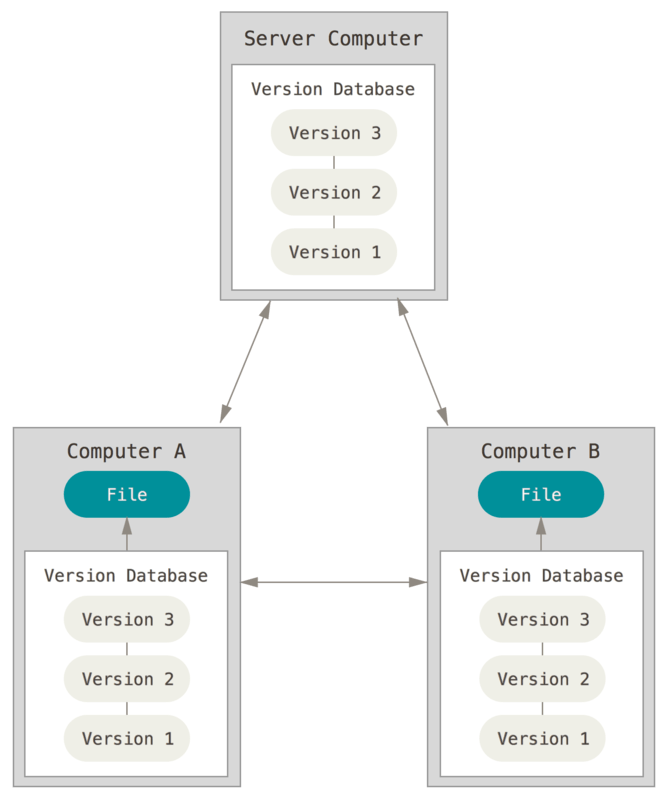
\includegraphics[height=0.7\textwidth]{./obrazki/fig-1_3.png}
   \footfullcite{pro_git}
 \end{center} 
\end{frame}


\section{Git}
\subsection{Historia}
\begin{frame}
 \frametitle{Jak zrodził się Git?}
GNU, jądra Linuxa, patches, BitKeeper \\
Linus Torvalds założył, że to nowe narzędzie powinno \\
  \begin{itemize}
  \item być dystrybuowalne
  \item unieść jądro Linuxa
  \item wspierać pracę nieliniową
 \end{itemize}
\end{frame}

\subsection{Istota}

\begin{frame}{Trzy fazy pracy Gita}{Committed, modified, staged}
 Wyróżniamy trzy etapy pracy w ramach lokalnego repozytorium
  \begin{center}
   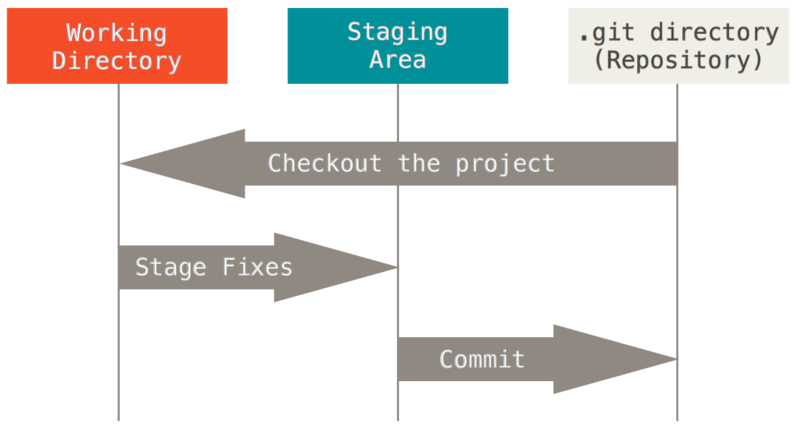
\includegraphics[width=0.8\textwidth]{./obrazki/fig-1_6.png}
   \footfullcite{pro_git}
 \end{center}
\end{frame}

\begin{frame}{Różnice w rozumieniu zmian w plikach}{Stream of snapshots vs diff}
  \begin{center}
   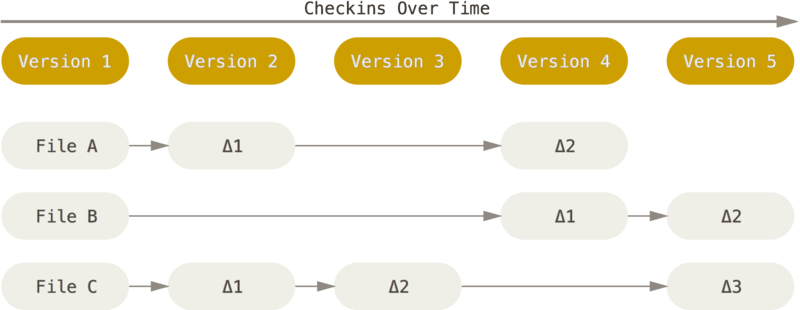
\includegraphics[width=0.6\textwidth]{./obrazki/fig-1_4.png}\\
   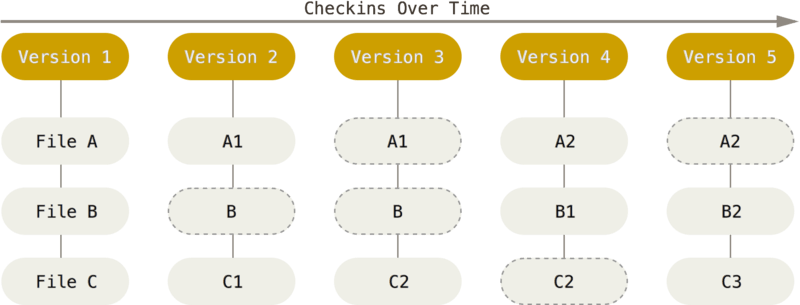
\includegraphics[width=0.6\textwidth]{./obrazki/fig-1_5.png}
   \footfullcite{pro_git}
 \end{center}

\end{frame}

\begin{frame}{Jak Git dostrzega zmiany?}
 Pliki hashuje się przy użyciu algorytmu \textbf{SHA-1}(Secure Hash Algorithm 1, zapis do 160 bitów, wyświetlanych w postaci 16-stkowej) \\
 
 Filozofia pointerów - wskaźnik Head, pochodne branch, pochodne commits.
\end{frame}

\subsection{Branch}
\begin{frame}{Branch}
   \begin{center}
   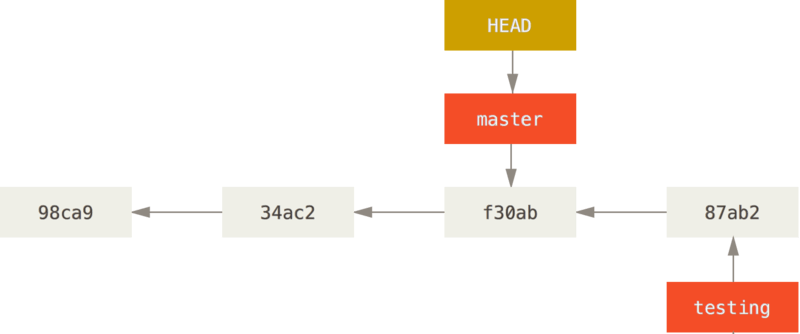
\includegraphics[width=0.8\textwidth]{./obrazki/fig-3_8.png}
   \footfullcite{pro_git}
 \end{center}
\end{frame}

\begin{frame}
Ciekawszy i bardziej pouczający przykład branch
   \begin{center}
   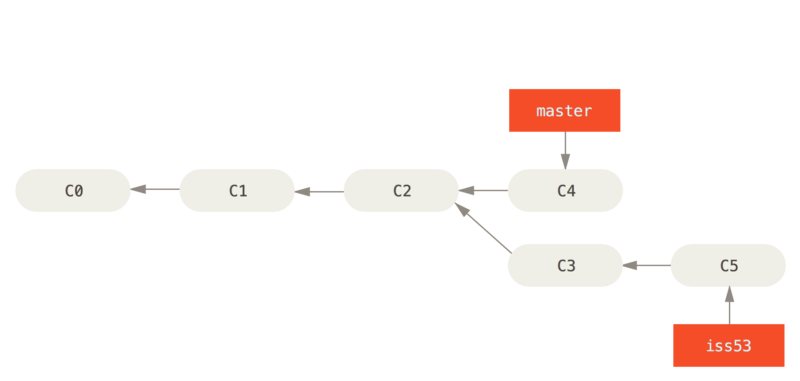
\includegraphics[width=0.8\textwidth]{./obrazki/fig-3_15.png}
   \footfullcite{pro_git}
 \end{center}
\end{frame}

\subsection{Merge}
\begin{frame}{Merge}
   \begin{center}
   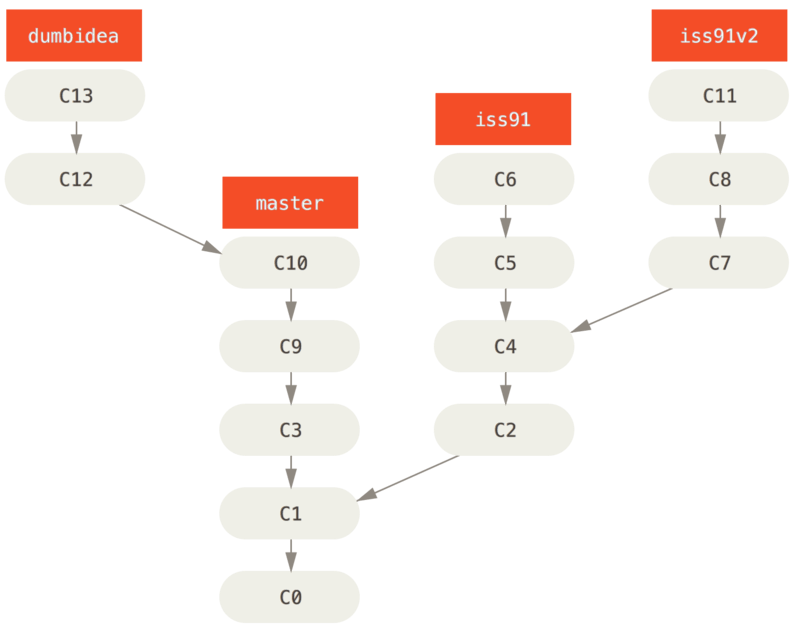
\includegraphics[width=0.8\textwidth]{./obrazki/fig-3_20.png}
   \footfullcite{pro_git}
 \end{center}
\end{frame}

\section{Obsługa Gita}

\subsection{Inicjalizacja repozytorium}
\begin{frame}{Jak stworzyć repozytorium}
 Dwie strategie
 \begin{itemize}
  \item Import istniejącego projektu \\
  \texttt{git init}
  \item Klon istniejącego już repozytorium gitowskiego \\
  \texttt{git clone https://github.com/libgit2/libgit2}
 \end{itemize}
\end{frame}

\subsection{Stage i commit}
\begin{frame}{Stage i commit}{Wyeksponuj i popełnij}
 
\end{frame}

\subsection{Obsługa branch}
\begin{frame}{Branch}{Zrównoleglij pracę}
 Podstawowe komendy:
 \begin{itemize}
  \item \texttt{git checkout -b branch0} - budowanie nowej gałęzi
  \item \texttt{git checkout  branch1} - przełączenie się na gałąź już istniejącą
  \item \texttt{git checkout -d branch1} - usuwanie gałęzi
  \item \texttt{git branch} - sprawdzanie na jakiej jestem gałęzi i jakie w ogóle istnieją [w moim drzewie?]
 \end{itemize}

\end{frame}

\section{Zalety}

\begin{frame}
\frametitle{Zalety}
\begin{itemize}
 \item Posiadanie pełnej historii we własnym repozytorium
 \item Commit popełnia się offline, a synchronizacja jest nieinteraktywna
 \item Dobrze zorganizowana praca na równoległych gałęziach
 \item Periodic explicit object packing
\end{itemize}
 
\end{frame}

\subsection{Rozmówki gitowskie}
\begin{frame}
 \frametitle{Savoir-vivre w Gitcie}
\end{frame}

\end{document}
